%%%%%%%%%%%%%%%%%%%%%%%%%%%%%%%%%%%%%%%%%%%%%%%%%%%%%%%%%%%%%%%%%%%%%%
% Dual Trace Communication Event Analysis
% 
% Author: Nora Huang
% Date: July 2017
% 
%%%%%%%%%%%%%%%%%%%%%%%%%%%%%%%%%%%%%%%%%%%%%%%%%%%%%%%%%%%%%%%%%%%%%%

\documentclass[paper=a4, fontsize=11pt]{scrartcl}
\usepackage[T1]{fontenc}
\usepackage{fourier}
\usepackage{tabu}
\usepackage{float}
\usepackage{afterpage}
\usepackage{booktabs}

\usepackage{longtable}
\usepackage{multicol}
\usepackage{multirow}

\usepackage[english]{babel}															% English language/hyphenation
\usepackage[protrusion=true,expansion=true]{microtype}	
\usepackage{amsmath,amsfonts,amsthm} % Math packages
\usepackage[pdftex]{graphicx}	
\usepackage{url}
\usepackage{listings}
\lstset{
    frame=single,
    breaklines=true
}


%%% Custom sectioning
\usepackage{sectsty}
\allsectionsfont{\centering \normalfont\scshape}


%%% Custom headers/footers (fancyhdr package)
\usepackage{fancyhdr}
\pagestyle{fancyplain}
\fancyhead{}											% No page header
\fancyfoot[L]{}											% Empty 
\fancyfoot[C]{}											% Empty
\fancyfoot[R]{\thepage}									% Pagenumbering
\renewcommand{\headrulewidth}{0pt}			% Remove header underlines
\renewcommand{\footrulewidth}{0pt}				% Remove footer underlines
\setlength{\headheight}{13.6pt}


%%% Equation and float numbering
\numberwithin{equation}{section}		% Equationnumbering: section.eq#
\numberwithin{figure}{section}			% Figurenumbering: section.fig#
\numberwithin{table}{section}				% Tablenumbering: section.tab#


%%% Maketitle metadata
\newcommand{\horrule}[1]{\rule{\linewidth}{#1}} 	% Horizontal rule

\title{
		%\vspace{-1in} 	
		\usefont{OT1}{bch}{b}{n}
		\normalfont \normalsize \textsc{Department of Computer Science,  University of Victoria} \\ [25pt]
		\horrule{0.5pt} \\[0.4cm]
		\huge Dual Trace Communication Event Analysis  \\
		\horrule{2pt} \\[0.5cm]
}
\author{
		\normalfont 								\normalsize
        Nora Huang\\[-3pt]		\normalsize
        \today
}
\date{}


%%% Begin document
\begin{document}
\maketitle

\section{Introduction}
Many network application vulnerabilities occur not just in one application, but in how they interact with other systems. These kinds of vulnerabilities can be difficult to analyze. Dual-trace analysis is one approach that helps the security engineers to detect the vulnerabilities in the interactive software. A dual-trace consist of two execution traces that are generated from two interacting applications. Each of these traces contains information including CPU instructions, register and memory changes of the running application. Communication information of the interacting applications is captured as the register or memory changes on their respective sides. Our research focuses on building a model to visualize and analyze dual-trace which would be available for various kinds of communication Type.

\section{Problem}
The major problem we are considering in dual-trace analysis is locating the synchronization point of the traces from both sides. We narrow down the problem into finding the sending points and receiving points of the communication messages and pair them. To do that in assembly level trace, there are three essential information to figure out: the messaging channel matching, individual message matching in each channel.

\section{Communication Types}
In order to synchronize the messaging of both side of the traces, we need to investigate the communication methods to figure out how they looks like in the assembly level traces.
There are so many communication methods exists in the real world. We are not covering all of them at a time, but start from narrowing down our study into some sort of communication methods. We start from investigating the messaging methods in Windows Communication Framework. There are two kinds of messaging channels in this framework, transport channels and protocol channel. We are current focus on transport channels. Transport channels read and write messages from the network (or some other communication point with the outside world). Example of transport channels are named pipes, MSMQ, HTTP and TCP channels. If our research turns out to be work in that particular communication methods, it is possible to extend it for more general use cases.
\subsection{Assembly Calling Convention}
Before we jumping into each communication method, it is important to know some basic assembly calling convention.
Calling Convention is different for operating system and the programming language. Since we are looking into the messaging methods being used in windows communication framework, and since our case study in running on a Microsoft* x64 system, we only list the Microsoft* x64 calling convention for interfacing with C/C++ style functions:\par
\begin{enumerate}  
\item RCX, RDX, R8, R9 are used for integer and pointer arguments in that order left to right.
\item XMM0, 1, 2, and 3 are used for floating point arguments.
\item Additional arguments are pushed on the stack left to right. \ldots 
\item Parameters less than 64 bits long are not zero extended; the high bits contain garbage.
\item Integer return values (similar to x86) are returned in RAX if 64 bits or less.
\item Floating point return values are returned in XMM0.
\item Larger return values (structs) have space allocated on the stack by the caller, and RCX then contains a pointer to the return space when the callee is called. Register usage for integer parameters is then pushed one to the right. RAX returns this address to the caller.
\end{enumerate}

\subsection{Named pipes Channel}
A named pipe is a named, one-way or duplex pipe for communication between the pipe server and one or more pipe clients. All instances of the named pipe share the same pipe name, but each instance has it own buffers and handlers. In here we only consider one to one server/client pairs. One server to multiple client scenario can always be divided into multiple server/client pairs cases. To define a Named Pipes message event, we need to know how the channels are created as well as how the messages are send and received in the traces. The creation of a channel will return the handler of that channel. This handler will be used later on when the message is send or receive. So we need to know the function calls for channel creation and message send/receive to located them in the traces. In the follow subsections, we will describe the related function for the named pipe channel for both synchronous mode and asynchronous mode. The create channel functions for both mode are the same but with different input parameters. The functions for send and receive message are also the same for both case. However, the operation of the send and receive functions are different for different mode. In addition, extra functions are being called to fully send or received the messages in asynchronous mode.
\subsubsection{Synchronous}
We list all the functions that needed to locate an messaging event in a dual-trace in Table\ref{synfunctions}. The Channel Create Functions indicate how the channel being created in sender and receiver sides, and the mattered parameters. For named pipes the channel create functions are different between the sender and receiver side. The parameter in RDX can indicate if the channel is opened as synchronous mode. The send or receive message functions are the same in both side. When the channel is being created, the input file name for a channel between sender and the receiver is the same, but the returned File Handler IDs are different. The send and receive function only use the handler to send and receive message to a specific channel. 
\begin{table}[h]
        \centering
        \caption{Named pipes system functions}
        \label{synfunctions}
        \begin{tabular}{|l|l|l|l|l|l|l|}
            \hline
             \multirow{2}{*}{} &
               \multicolumn{2}{c|}{Channel Create Functions} &
               \multicolumn{2}{c|}{Message Send Functions} &
               \multicolumn{2}{c|}{Message Receive Functions} \\
             \cline{2-7}
              & Function& Parameters & Function & Parameters  & Function & Parameters\\
             \hline
             Sever& Create-&  RAX: File Handler &  &  RCX: File Handler &&RCX: File Handler\\
             \cline{3-3} \cline{5-5} \cline{7-7}
             &NamedPipe&RCX: File Name && RDX:  &&RDX: \\
              \cline{3-3} 
             &&RDX: Asyn/Syn&ReadFile& Buffer Address &WriteFile&Buffer Address\\
                \cline{1-3} \cline{5-5} \cline{7-7}
             Client & CreateFile & RAX: File Handler & &  R8: Buffer Length &&R8: Buffer Length\\
              \cline{3-3} \cline{5-5} \cline{7-7}
             &&RCX: File Name &&Stack:&&Stack:\\
             \cline{3-3} 
             &&RDX: Asyn/Syn&& Overlap Pointer&&Overlap Pointer\\
            \hline
        \end{tabular}
    \end{table}
\subsubsection{Asynchronous}
The functions used in Asynchronous mode for create channel, send and receive message are the same. However, for the the ReadFile and WriteFile functions run asynchronously when the channel is asynchronous. This means the function will return immediately, even if the operation has not been completed. If the operation is complete when the function returns, the return value indicates the success or failure of the operation. Otherwise the functions return zero and GetLastError returns ERROR_IO_PENDING. In this case, the calling thread must wait until the operation has finished. The calling thread must then call the GetOverlappedResult function to determine the results. This means besides looking for ReadFile and WriteFile function calls in the traces, the GetOverlappedResult function should be checked in the traces to get the full result of the ReadFile or WriteFile operations. Table\ref{asynfunctions} list the interested parameters of the GetOverlappedResult function.
\begin{table}[h]
        \centering
        \caption{Named pipes system functions}
        \label{asynfunctions}
        \begin{tabular}{|l|l|l|l|l|l|l|}
            \hline
             \multirow{2}{*}{} &
               \multicolumn{2}{c|}{Channel Create Functions} &
               \multicolumn{2}{c|}{Message Send Functions} &
               \multicolumn{2}{c|}{Message Receive Functions} \\
             \cline{2-7}
              & Function& Parameters & Function & Parameters  & Function & Parameters\\
             \hline
             Sever& Create-&  RAX: File Handler &  &  RCX: File Handler &&RCX: File Handler\\
             \cline{3-3} \cline{5-5} \cline{7-7}
             &NamedPipe&RCX: File Name && RDX:  &&RDX: \\
              \cline{3-3} 
             &&RDX: Asyn/Syn&ReadFile& Buffer Address &WriteFile&Buffer Address\\
                \cline{1-3} \cline{5-5} \cline{7-7}
             Client & CreateFile & RAX: File Handler & &  R8: Buffer Length &&R8: Buffer Length\\
              \cline{3-3} \cline{5-5} \cline{7-7}
             &&RCX: File Name &&Stack:&&Stack:\\
             \cline{3-3} 
             &&RDX: Asyn/Syn&& Overlap Pointer&&Overlap Pointer\\
            \hline
        \end{tabular}
    \end{table}
\subsection{MSMQ Channel}
\subsection{HTTP Channel}
\subsection{TCP Channel}


\section{Prototype Building}
In this section we discuss the design of the prototype on how we match the send and receive events in the sender side trace and the receiver side trace. This prototype consist of three main components: defining the communication type, locating the communication events by matching the send and receive events on sender and receiver sides, navigating the located events in the sender and receiver traces. We provide the background information of the design of each component as well as its detail design in each corresponding subsection.
\subsection{User Defined Communication Type}
In our design, we don't specify any predefined communication type but give the user capacity to do that. By the user interface implemented in our tool, the user can defined their own communication type. This give the flexibility to the user to define what they are looking for. Each communication type consist of 4 system function calls. They are sender and receiver channel create/open, sender's send message function and receiver's receive message function. By indicating these the channel create/open function in both sender and receiver sides, the tool can acquire the channel's identifiers when they are created or opened. Later on the tool can match the send and received messages within a specific channel. The send and receive are used to located the event happened in the traces. The messages send and received are reconstructed from the memory state when the send and receive functions are called and returned. This detail of the match algorithm will be discuss later.

\subsubsection{Function Calls in the Traces}
The called functions' name can be inspected  by  search of the symbolic name in the executable binary or any DLLs which used by the program at the time when it is traced. This functionality exists in the current Atlantis. By importing the Dlls and execution  executable binary, Atlantis can list all called functions for the users in the Functions view. From this list, users can chose the interested functions and generate their interested communication type. In Figure\ref{functionsview} there is  an action item call "Add to Communication type" in the right click menu of the function entry. Figure \ref{dialog} shows the dialogue for entering the information for the added function. The needed information is the communication type's name. User can get the existing communication type list in the drop down menu. They can choose to add the current function to an exist communication type or they can add it to a new communication type by entering a new name. For the channel create/open function, the register holding the address of channel's name as input and the register holding the handle identification of the channel as output are required. For the send/receive function, the register holding the address of the send/receiver buffer, the register holding the length of the sending/receiving message and the register holding the channel's identification are required. As there are 4 functions for each communication type the user has to repeat this add function to communication type action for 4 time to generate one communication type.

\begin{figure}[h]
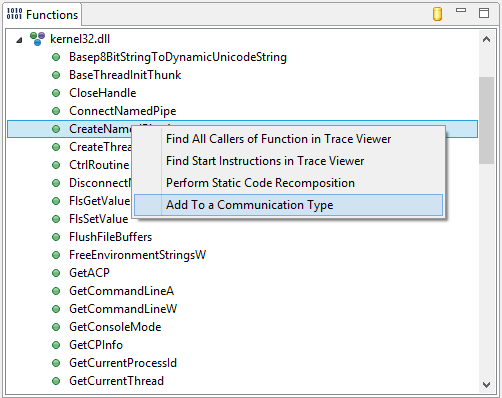
\includegraphics{functionsview}
 \caption{Add function to a Communication type from Functions View}
\label{functionsview}
\end{figure}

\begin{figure}[h]
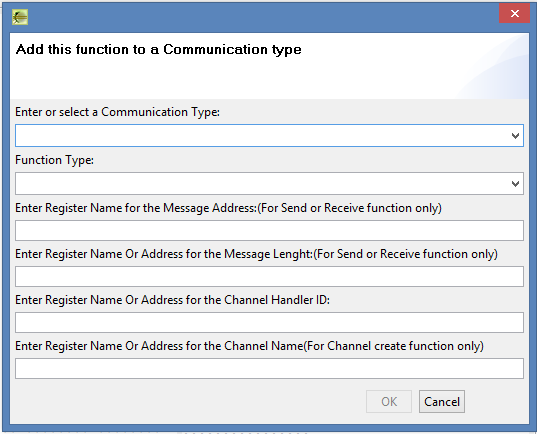
\includegraphics{dialog}
 \caption{Dialog to input information for a function adding to a communication type}
\label{dialog}
\end{figure}

\subsubsection{Communication Type Data Structure}
The defined communication type will be stored in a xml file. The list below shows the data structure of one communication type. 
\begin{lstlisting}
<messageTypesData>
    <parentFolder>.tmp</parentFolder>
    <messageTypes>
        <messageType>
            <name>namedPipe_clientsend</name>
            <sendFunction>
                <associatedFileName>Client</associatedFileName>
                <name>WriteFile</name>
                <messageAddress>RDX</messageAddress>
                <messageLengthAddress>R8</messageLengthAddress>
                <channelIdReg>RCX</channelIdReg>
            </sendFunction>
            <receiveFunction>
                <associatedFileName>Server</associatedFileName>
                <name>ReadFile</name>
                <messageAddress>RDX</messageAddress>
                <messageLengthAddress>R8</messageLengthAddress>
                <channelIdReg>RCX</channelIdReg>
            </receiveFunction>
            <sendChannelCreateFunction>
                <associatedFileName>Client</associatedFileName>
                <name>CreateFileA</name>
                <channelIdReg>RAX</channelIdReg>
                <channelNameAddress>RCX</channelNameAddress>
            </sendChannelCreateFunction>
            <receiveChannelCreateFunction>
                <associatedFileName>Server</associatedFileName>
                <name>CreateNamedPipeA</name>
                <channelIdReg>RAX</channelIdReg>
                <channelNameAddress>RCX</channelNameAddress>
            </receiveChannelCreateFunction>
        </messageType>
    </messageTypes>
</messageTypesData>
\end{lstlisting}


\subsubsection{Communication Type View}
A new view named Communication Types view is for the user defined communication types. All user defined communication type are listed in this view  as shown in Figure \ref{CommunicationTypeview}. User can change the name of a communication type, remove an existing communication type or searching of the match message occurrences of selected communication type by selecting the selected action item in the right click menu of an communication type entry. The matched messages are listed in the sub window of the view. By clicking the entry of the search  result, user can navigate to it's sender or receiver's corresponding instruction line as shown in Figure\ref{searchresult}. Message content in the memory view will be shown as well.


\begin{figure}[h]
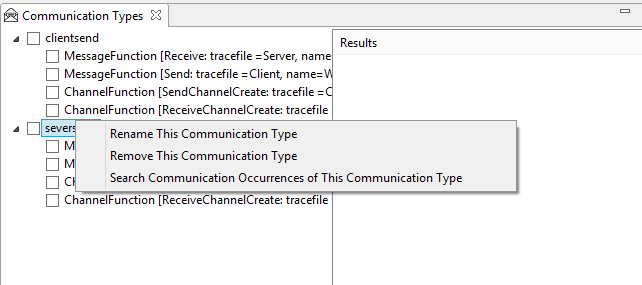
\includegraphics{CommunicationTypeview}
 \caption{New View: Communication Type View}
\label{CommunicationTypeview}
\end{figure}

\begin{figure}[h]
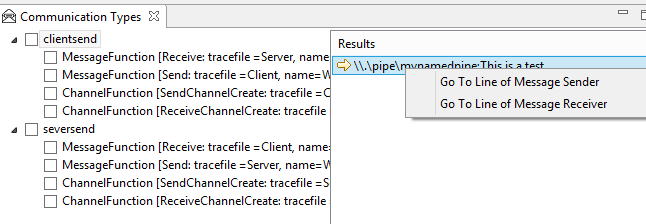
\includegraphics{searchresult}
 \caption{Right Click menu to navigate to send and receive event in the traces}
\label{searchresult}
\end{figure}

\subsection{Communication Event Searching}
The communication Event consists of the send message event in the sender side and receive message event in the receiver side. The communication event searching algorithm can be divided into three main steps: 1. search all channel create/open event in the sender and receiver side, save the handle id and corresponding channel name. 2. Search all message send and receive event in sender and receiver sides. 3. Matching the send/receive messages pair based on the channel names and message contents.
\subsubsection{Record opened Channel}

\subsubsection{Search send and receive Message}
\subsubsection{Matching the send/receive messages pair}
\subsubsection{Matching Event Data Structure}
\begin{table}[h]
 \begin{center}
  \caption{Matched message pair data structure}
\label{table2}
\begin{tabular}{|c|c|c|c|c|}
      \hline
         Message& sender function name & sender line number  & receiver function name & receiver line number \\
       \hline
\end{tabular}
\end{center}
\end{table}
\subsection{Matching Event Visualization and Navigation}
\subsubsection{Navigating to The Sender/Receiver}
\subsubsection{Message Shown in memory view}


\section{Case Study}
Our prototype only be tested on traces of Microsoft 64 with C/C++ program. It seems too specific, however, the prototype can be adapted easily to other conventions. As long as users know the calling convention of their operating system, they can define their communication type with our tool. We list the related Microsoft 64 with C/C++ program convention here for reference and example. For more detail about the calling convention, users should refer to the operating system specification.\par
\subsubsection{communication type definition}

\subsection{Experiment Design}
\subsection{Result}
\subsection{Time Analysis}
\section{Limitations}
In this section, we specify the limitations of the current prototype and the reasons for them. 
\subsection{Named pipes Channel}
\subsubsection{Event Status: Success or Fail}
In current prototype, we only consider the success cases. For the Fail case, since the message was not successfully sent or received, there are high chance that they are not existed in the memory of the trace. From the assembly level trace, if the message was not traced in the memory, there is no way to match the sent/received message pair in the trace analysis.   
\subsubsection{Match Events Distinguishing}
Distinguishing is considered when multiple clients connecting to the same server. Each connection is considered as an instance. In the server side all this instances have the same pipe name but different handler ID. However in the assembly trace level there is no way to match a client with it instance handler ID. In consequence, if the same content messages are being sent/received by different clients, when the user want to match the message pair between a client and the server, there is no way to distinguish the correct one from the assembly trace level. As a result, our tool will list all the matched content message event, regardless if it's from the interested client. The user can distinguish the correct ones for this client, if they have extra information.

\subsubsection{Match Events Ordering}
Ordering is considered when multiple messages with exactly the same content being send/receive between the client and server. If the channel is synchronous, the order of the event is always consist with the order they happen in both the sender and receive sides. However for the asynchronous channel, there are chance that the sent messages in the sender side's trace are out of order with the received messages in the received side's trace. Unfortunately, There is no way in the assembly level trace to match the exactly ones. As a result, our tool can only order the event based on the order they happen in the traces.
\section{Future Work}


\bibliographystyle{abbrv}
\bibliography{referencelist} 


%%% End document
\end{document}